
\lecture{Hypothesis Testing With The Sample Standard Deviation}{hypothesis-testing-single-sample}
\section{Hypothesis Testing With The Sample Standard Deviation}

\title{Hypothesis Testing}
\subtitle{What if you do not know the true standard deviation?}

%\author{Kelly Black}
%\institute{Clarkson University}
\date{13 March 2015}

\begin{frame}
  \titlepage
\end{frame}

\begin{frame}
  \frametitle{Outline}
  \tableofcontents[hideothersubsections,sectionstyle=show/hide]
\end{frame}


\subsection{Clicker Quiz}

\iftoggle{clicker}{%
  \begin{frame}{Clicker Quiz}

    \iftoggle{clicker}{%

      \begin{eqnarray*}
        \begin{array}{lrcl}
          H_0: & \mu & = & 45.0 \\
          H_a: & \mu & \neq & 45.0
        \end{array}
      \end{eqnarray*}

      \begin{eqnarray*}
        n & = & 10, \\
        \bar{x} & = & 49.9,\\
        \sigma & = & 8.0, \\
        \alpha & = & 0.05.
      \end{eqnarray*}

      \vfill 

      What is the \textit{critical} $z$-statistic?

      \begin{tabular}{l@{\hspace{3em}}l@{\hspace{3em}}l@{\hspace{3em}}l}
        A: 0.613  & B: 1.64 & C: 1.94  & D: 1.96 
      \end{tabular}

      \vfill
      \vfill
      \vfill

    }

  \end{frame}

}






\subsection{Hypothesis Testing}

\begin{frame}
  \frametitle{Left Sided Test of the Mean}

  You think that the mean is lower.

  \begin{columns}
    \column{0.25\textwidth}
    \begin{eqnarray*}
      \begin{array}{lrcl}
        H_0: & \mu & = & \# \\
        H_a: & \mu & < & \#
      \end{array}
    \end{eqnarray*}

    \column{0.75\textwidth}

    \includegraphics[width=5cm]{img/leftSideHypothesisTest}

  \end{columns}

  \begin{description}
  \item[$p$-value Approach] The probability that you do worse than
    $\bar{x}$ is the area to the left under the curve. If the area is
    smaller than the significance level ($\alpha$) then it is an
    \textit{unlikely result}.
  \item[Classical Approach] The area to the left of $x_{cr}$ is
    equal to the significance level ($\alpha$). If your $\bar{x}$ is
    less than this critical value then it is an \textit{unlikely
      result}.
  \end{description}


\end{frame}

\begin{frame}
  \frametitle{Right Sided Test of the Mean}

  You think that the mean is higher.

  \begin{columns}
    \column{0.25\textwidth}
    \begin{eqnarray*}
      \begin{array}{lrcl}
        H_0: & \mu & = & \# \\
        H_a: & \mu & > & \#
      \end{array}
    \end{eqnarray*}

    \column{0.75\textwidth}

    \includegraphics[width=5cm]{img/rightSideHypothesisTest}

  \end{columns}

  \begin{description}
  \item[$p$-value Approach] The probability that you do worse than
    $\bar{x}$ is the area to the right under the curve. If the area is
    smaller than the significance level ($\alpha$) then it is an
    \textit{unlikely result}.
  \item[Classical Approach] The area to the right of $x_{cr}$ is
    equal to the significance level ($\alpha$). If your $\bar{x}$ is
    more than this critical value then it is an \textit{unlikely
      result}.
  \end{description}


\end{frame}


\begin{frame}
  \frametitle{Two Sided Test of the Mean}

  \vspace*{-1em}

  You think that the mean is different.

  \begin{columns}
    \column{0.25\textwidth}
    \begin{eqnarray*}
      \begin{array}{lrcl}
        H_0: & \mu & = & \# \\
        H_a: & \mu & \neq & \#
      \end{array}
    \end{eqnarray*}

    \column{0.75\textwidth}

    \includegraphics[width=5cm]{img/twoSideHypothesisTest}

  \end{columns}

  \begin{description}
  \item[$p$-value Approach] The probability that you do worse than
    $\bar{x}$ is the area to the left \textit{and} right under the
    curve. If the area is smaller than the significance level
    ($\alpha$) then it is an \textit{unlikely result}.
  \item[Classical Approach] The area to the left of
    $\mu-\mathrm{error}$ and to the right of $\mu+\mathrm{error}$ is
    equal to the significance level ($\alpha$). If your $\bar{x}$ is
    less than $\mu-\mathrm{error}$ or more than $\mu+\mathrm{error}$
    this critical value then it is an \textit{unlikely result}.
  \end{description}


\end{frame}


\begin{frame}{The Possibilities}

  \centerline{\includegraphics[width=3.0cm]{img/hindenburg}}

  \begin{eqnarray*}
    \mathrm{Data~-} & &
      \begin{array}{l@{\hspace{1em}}|c|c|} 
        \multicolumn{3}{r}{\mathrm{Reality}} \\ 
        \multicolumn{1}{c}{~} & \multicolumn{1}{c}{H_0
          \mathrm{~is~true}} & \multicolumn{1}{c}{H_0
          \mathrm{~is~false}} \\  
        \hhline{~--}
        \mathrm{Do~Not~Reject~}H_0 & \includegraphics[width=0.7cm]{img/smiley} & \mathrm{Type~II~Error} \\ \hhline{~|-|-|}
        \mathrm{Reject~}H_0 & \mathrm{Type~I~Error} & \includegraphics[width=0.7cm]{img/smiley} \\ \hhline{~--}
      \end{array}
  \end{eqnarray*}
  
\end{frame}




\iftoggle{clicker}{%
  \begin{frame}
    \frametitle{Clicker Quiz}

    A supermarket estimates that the mean time spent by customers in a
    store for each visit is about 23.4 minutes with a standard
    deviation of 11.2 minutes. They rearrange one aisle, monitor the
    times for eighteen randomly chosen people, and find a sample mean
    of 27.9 minutes. Did the mean time per visit increase? (Use a 5\%
    significance level.)

    \begin{eqnarray*}
      \begin{array}{lrcl}
        H_0: & \mu & = & 23.4 \\
        H_a: & \mu & > & 23.4
      \end{array}
    \end{eqnarray*}

    The $z$-statistic is 
    \begin{eqnarray*}
      z^* & = & \frac{27.9-23.4}{11.2/\sqrt{18}}, \\
      & \approx & 1.70
    \end{eqnarray*}

    \vfill

    \begin{tabular}{l@{\hspace{3em}}l@{\hspace{3em}}l@{\hspace{3em}}l}
      A: Reject $H_0$  & B: Cannot reject $H_0$
    \end{tabular}

    \vfill
    \vfill
    \vfill

  \end{frame}
}



\subsection{Recall: t-Distribution}

\begin{frame}
  \frametitle{Problem!}

  There is a problem.

  \only<2->
  {
    We do not know $\sigma$!
  }

  \only<3->
  {
    If you \textbf{trust} your \textit{estimate} for $\sigma$ then
    what we did is fine.
  }

  \only<4->
  {
    What if you only have $s$?
  }


  \only<5->
  {
    use the $t$-distribution, of course!
  }


\end{frame}


\begin{frame}
  \frametitle{Decisions, Decisions, Decisions...}

  % Graphic for TeX using PGF
% Title: /home/black/write/class/stat/stat282-12/class/img/confidenceIntervalDist.dia
% Creator: Dia v0.97.2
% CreationDate: Mon Mar  4 12:17:58 2013
% For: black
% \usepackage{tikz}
% The following commands are not supported in PSTricks at present
% We define them conditionally, so when they are implemented,
% this pgf file will use them.
\ifx\du\undefined
  \newlength{\du}
\fi
\setlength{\du}{15\unitlength}
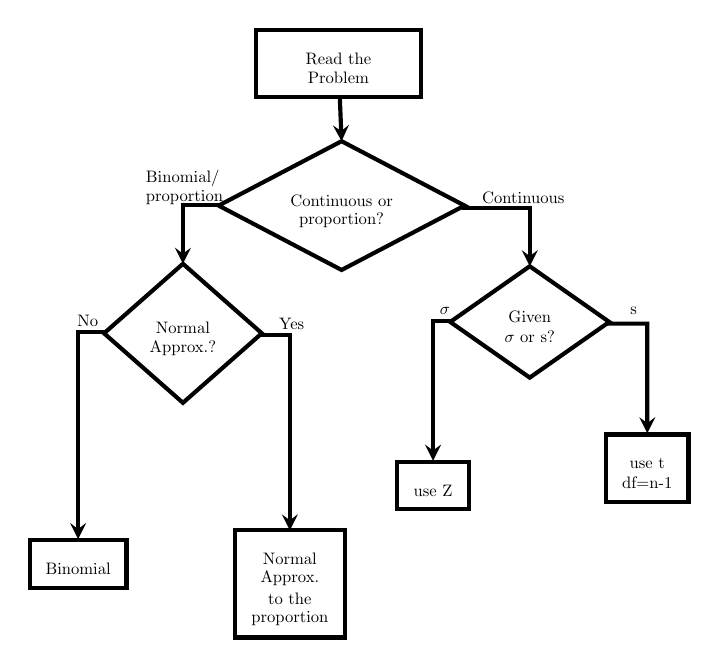
\begin{tikzpicture}[thick,scale=0.6, every node/.style={scale=0.6}]
\pgftransformxscale{1.000000}
\pgftransformyscale{-1.000000}
\definecolor{dialinecolor}{rgb}{0.000000, 0.000000, 0.000000}
\pgfsetstrokecolor{dialinecolor}
\definecolor{dialinecolor}{rgb}{1.000000, 1.000000, 1.000000}
\pgfsetfillcolor{dialinecolor}
\definecolor{dialinecolor}{rgb}{1.000000, 1.000000, 1.000000}
\pgfsetfillcolor{dialinecolor}
\fill (9.875000\du,2.350000\du)--(9.875000\du,5.050000\du)--(16.525000\du,5.050000\du)--(16.525000\du,2.350000\du)--cycle;
\pgfsetlinewidth{0.100000\du}
\pgfsetdash{}{0pt}
\pgfsetdash{}{0pt}
\pgfsetmiterjoin
\definecolor{dialinecolor}{rgb}{0.000000, 0.000000, 0.000000}
\pgfsetstrokecolor{dialinecolor}
\draw (9.875000\du,2.350000\du)--(9.875000\du,5.050000\du)--(16.525000\du,5.050000\du)--(16.525000\du,2.350000\du)--cycle;
% setfont left to latex
\definecolor{dialinecolor}{rgb}{0.000000, 0.000000, 0.000000}
\pgfsetstrokecolor{dialinecolor}
\node at (13.200000\du,3.495000\du){Read the };
% setfont left to latex
\definecolor{dialinecolor}{rgb}{0.000000, 0.000000, 0.000000}
\pgfsetstrokecolor{dialinecolor}
\node at (13.200000\du,4.295000\du){Problem};
\pgfsetlinewidth{0.100000\du}
\pgfsetdash{}{0pt}
\pgfsetdash{}{0pt}
\pgfsetbuttcap
{
\definecolor{dialinecolor}{rgb}{0.000000, 0.000000, 0.000000}
\pgfsetfillcolor{dialinecolor}
% was here!!!
\pgfsetarrowsend{stealth}
\definecolor{dialinecolor}{rgb}{0.000000, 0.000000, 0.000000}
\pgfsetstrokecolor{dialinecolor}
\draw (13.257154\du,5.099002\du)--(13.327646\du,6.824488\du);
}
\pgfsetlinewidth{0.100000\du}
\pgfsetdash{}{0pt}
\pgfsetdash{}{0pt}
\pgfsetmiterjoin
\pgfsetbuttcap
{
\definecolor{dialinecolor}{rgb}{0.000000, 0.000000, 0.000000}
\pgfsetfillcolor{dialinecolor}
% was here!!!
\pgfsetarrowsend{stealth}
{\pgfsetcornersarced{\pgfpoint{0.000000\du}{0.000000\du}}\definecolor{dialinecolor}{rgb}{0.000000, 0.000000, 0.000000}
\pgfsetstrokecolor{dialinecolor}
\draw (8.390350\du,9.409510\du)--(8.390350\du,9.400000\du)--(6.958340\du,9.400000\du)--(6.958340\du,11.745900\du);
}}
\definecolor{dialinecolor}{rgb}{1.000000, 1.000000, 1.000000}
\pgfsetfillcolor{dialinecolor}
\fill (6.958337\du,11.745900\du)--(10.124835\du,14.536969\du)--(6.958337\du,17.328039\du)--(3.791840\du,14.536969\du)--cycle;
\pgfsetlinewidth{0.100000\du}
\pgfsetdash{}{0pt}
\pgfsetdash{}{0pt}
\pgfsetmiterjoin
\definecolor{dialinecolor}{rgb}{0.000000, 0.000000, 0.000000}
\pgfsetstrokecolor{dialinecolor}
\draw (6.958337\du,11.745900\du)--(10.124835\du,14.536969\du)--(6.958337\du,17.328039\du)--(3.791840\du,14.536969\du)--cycle;
% setfont left to latex
\definecolor{dialinecolor}{rgb}{0.000000, 0.000000, 0.000000}
\pgfsetstrokecolor{dialinecolor}
\node at (6.958337\du,14.331969\du){Normal};
% setfont left to latex
\definecolor{dialinecolor}{rgb}{0.000000, 0.000000, 0.000000}
\pgfsetstrokecolor{dialinecolor}
\node at (6.958337\du,15.131969\du){Approx.?};
% setfont left to latex
\definecolor{dialinecolor}{rgb}{0.000000, 0.000000, 0.000000}
\pgfsetstrokecolor{dialinecolor}
\node[anchor=west] at (7.592530\du,9.700000\du){};
\definecolor{dialinecolor}{rgb}{1.000000, 1.000000, 1.000000}
\pgfsetfillcolor{dialinecolor}
\fill (13.327646\du,6.824488\du)--(18.264943\du,9.409510\du)--(13.327646\du,11.994531\du)--(8.390350\du,9.409510\du)--cycle;
\pgfsetlinewidth{0.100000\du}
\pgfsetdash{}{0pt}
\pgfsetdash{}{0pt}
\pgfsetmiterjoin
\definecolor{dialinecolor}{rgb}{0.000000, 0.000000, 0.000000}
\pgfsetstrokecolor{dialinecolor}
\draw (13.327646\du,6.824488\du)--(18.264943\du,9.409510\du)--(13.327646\du,11.994531\du)--(8.390350\du,9.409510\du)--cycle;
% setfont left to latex
\definecolor{dialinecolor}{rgb}{0.000000, 0.000000, 0.000000}
\pgfsetstrokecolor{dialinecolor}
\node at (13.327646\du,9.204510\du){Continuous or};
% setfont left to latex
\definecolor{dialinecolor}{rgb}{0.000000, 0.000000, 0.000000}
\pgfsetstrokecolor{dialinecolor}
\node at (13.327646\du,10.004510\du){proportion?};
% setfont left to latex
\definecolor{dialinecolor}{rgb}{0.000000, 0.000000, 0.000000}
\pgfsetstrokecolor{dialinecolor}
\node[anchor=west] at (5.200000\du,8.300000\du){Binomial/};
% setfont left to latex
\definecolor{dialinecolor}{rgb}{0.000000, 0.000000, 0.000000}
\pgfsetstrokecolor{dialinecolor}
\node[anchor=west] at (5.200000\du,9.100000\du){proportion};
\definecolor{dialinecolor}{rgb}{1.000000, 1.000000, 1.000000}
\pgfsetfillcolor{dialinecolor}
\fill (20.882209\du,11.845300\du)--(24.073819\du,14.081125\du)--(20.882209\du,16.316950\du)--(17.690600\du,14.081125\du)--cycle;
\pgfsetlinewidth{0.100000\du}
\pgfsetdash{}{0pt}
\pgfsetdash{}{0pt}
\pgfsetmiterjoin
\definecolor{dialinecolor}{rgb}{0.000000, 0.000000, 0.000000}
\pgfsetstrokecolor{dialinecolor}
\draw (20.882209\du,11.845300\du)--(24.073819\du,14.081125\du)--(20.882209\du,16.316950\du)--(17.690600\du,14.081125\du)--cycle;
% setfont left to latex
\definecolor{dialinecolor}{rgb}{0.000000, 0.000000, 0.000000}
\pgfsetstrokecolor{dialinecolor}
\node at (20.882209\du,13.876125\du){Given };
% setfont left to latex
\definecolor{dialinecolor}{rgb}{0.000000, 0.000000, 0.000000}
\pgfsetstrokecolor{dialinecolor}
\node at (20.882209\du,14.676125\du){$\sigma$ or s?};
% setfont left to latex
\definecolor{dialinecolor}{rgb}{0.000000, 0.000000, 0.000000}
\pgfsetstrokecolor{dialinecolor}
\node[anchor=west] at (20.882200\du,14.081100\du){};
\pgfsetlinewidth{0.100000\du}
\pgfsetdash{}{0pt}
\pgfsetdash{}{0pt}
\pgfsetmiterjoin
\pgfsetbuttcap
{
\definecolor{dialinecolor}{rgb}{0.000000, 0.000000, 0.000000}
\pgfsetfillcolor{dialinecolor}
% was here!!!
\pgfsetarrowsend{stealth}
{\pgfsetcornersarced{\pgfpoint{0.000000\du}{0.000000\du}}\definecolor{dialinecolor}{rgb}{0.000000, 0.000000, 0.000000}
\pgfsetstrokecolor{dialinecolor}
\draw (18.264943\du,9.409510\du)--(18.264943\du,9.500000\du)--(20.882200\du,9.500000\du)--(20.882200\du,11.845300\du);
}}
\definecolor{dialinecolor}{rgb}{1.000000, 1.000000, 1.000000}
\pgfsetfillcolor{dialinecolor}
\fill (15.563800\du,19.700000\du)--(15.563800\du,21.600000\du)--(18.436300\du,21.600000\du)--(18.436300\du,19.700000\du)--cycle;
\pgfsetlinewidth{0.100000\du}
\pgfsetdash{}{0pt}
\pgfsetdash{}{0pt}
\pgfsetmiterjoin
\definecolor{dialinecolor}{rgb}{0.000000, 0.000000, 0.000000}
\pgfsetstrokecolor{dialinecolor}
\draw (15.563800\du,19.700000\du)--(15.563800\du,21.600000\du)--(18.436300\du,21.600000\du)--(18.436300\du,19.700000\du)--cycle;
% setfont left to latex
\definecolor{dialinecolor}{rgb}{0.000000, 0.000000, 0.000000}
\pgfsetstrokecolor{dialinecolor}
\node at (17.000050\du,20.845000\du){use Z};
\definecolor{dialinecolor}{rgb}{1.000000, 1.000000, 1.000000}
\pgfsetfillcolor{dialinecolor}
\fill (23.943800\du,18.600000\du)--(23.943800\du,21.300000\du)--(27.256300\du,21.300000\du)--(27.256300\du,18.600000\du)--cycle;
\pgfsetlinewidth{0.100000\du}
\pgfsetdash{}{0pt}
\pgfsetdash{}{0pt}
\pgfsetmiterjoin
\definecolor{dialinecolor}{rgb}{0.000000, 0.000000, 0.000000}
\pgfsetstrokecolor{dialinecolor}
\draw (23.943800\du,18.600000\du)--(23.943800\du,21.300000\du)--(27.256300\du,21.300000\du)--(27.256300\du,18.600000\du)--cycle;
% setfont left to latex
\definecolor{dialinecolor}{rgb}{0.000000, 0.000000, 0.000000}
\pgfsetstrokecolor{dialinecolor}
\node at (25.600050\du,19.745000\du){use t};
% setfont left to latex
\definecolor{dialinecolor}{rgb}{0.000000, 0.000000, 0.000000}
\pgfsetstrokecolor{dialinecolor}
\node at (25.600050\du,20.545000\du){df=n-1};
\pgfsetlinewidth{0.100000\du}
\pgfsetdash{}{0pt}
\pgfsetdash{}{0pt}
\pgfsetmiterjoin
\pgfsetbuttcap
{
\definecolor{dialinecolor}{rgb}{0.000000, 0.000000, 0.000000}
\pgfsetfillcolor{dialinecolor}
% was here!!!
\pgfsetarrowsend{stealth}
{\pgfsetcornersarced{\pgfpoint{0.000000\du}{0.000000\du}}\definecolor{dialinecolor}{rgb}{0.000000, 0.000000, 0.000000}
\pgfsetstrokecolor{dialinecolor}
\draw (17.690600\du,14.081100\du)--(17.690600\du,14.050000\du)--(17.000042\du,14.050000\du)--(17.000049\du,19.650171\du);
}}
\pgfsetlinewidth{0.100000\du}
\pgfsetdash{}{0pt}
\pgfsetdash{}{0pt}
\pgfsetmiterjoin
\pgfsetbuttcap
{
\definecolor{dialinecolor}{rgb}{0.000000, 0.000000, 0.000000}
\pgfsetfillcolor{dialinecolor}
% was here!!!
\pgfsetarrowsend{stealth}
{\pgfsetcornersarced{\pgfpoint{0.000000\du}{0.000000\du}}\definecolor{dialinecolor}{rgb}{0.000000, 0.000000, 0.000000}
\pgfsetstrokecolor{dialinecolor}
\draw (24.073800\du,14.081100\du)--(24.073800\du,14.150000\du)--(25.600038\du,14.150000\du)--(25.600047\du,18.550269\du);
}}
\definecolor{dialinecolor}{rgb}{1.000000, 1.000000, 1.000000}
\pgfsetfillcolor{dialinecolor}
\fill (0.807500\du,22.850000\du)--(0.807500\du,24.750000\du)--(4.692500\du,24.750000\du)--(4.692500\du,22.850000\du)--cycle;
\pgfsetlinewidth{0.100000\du}
\pgfsetdash{}{0pt}
\pgfsetdash{}{0pt}
\pgfsetmiterjoin
\definecolor{dialinecolor}{rgb}{0.000000, 0.000000, 0.000000}
\pgfsetstrokecolor{dialinecolor}
\draw (0.807500\du,22.850000\du)--(0.807500\du,24.750000\du)--(4.692500\du,24.750000\du)--(4.692500\du,22.850000\du)--cycle;
% setfont left to latex
\definecolor{dialinecolor}{rgb}{0.000000, 0.000000, 0.000000}
\pgfsetstrokecolor{dialinecolor}
\node at (2.750000\du,23.995000\du){Binomial};
\definecolor{dialinecolor}{rgb}{1.000000, 1.000000, 1.000000}
\pgfsetfillcolor{dialinecolor}
\fill (9.032500\du,22.450000\du)--(9.032500\du,26.750000\du)--(13.467500\du,26.750000\du)--(13.467500\du,22.450000\du)--cycle;
\pgfsetlinewidth{0.100000\du}
\pgfsetdash{}{0pt}
\pgfsetdash{}{0pt}
\pgfsetmiterjoin
\definecolor{dialinecolor}{rgb}{0.000000, 0.000000, 0.000000}
\pgfsetstrokecolor{dialinecolor}
\draw (9.032500\du,22.450000\du)--(9.032500\du,26.750000\du)--(13.467500\du,26.750000\du)--(13.467500\du,22.450000\du)--cycle;
% setfont left to latex
\definecolor{dialinecolor}{rgb}{0.000000, 0.000000, 0.000000}
\pgfsetstrokecolor{dialinecolor}
\node at (11.250000\du,23.595000\du){Normal};
% setfont left to latex
\definecolor{dialinecolor}{rgb}{0.000000, 0.000000, 0.000000}
\pgfsetstrokecolor{dialinecolor}
\node at (11.250000\du,24.395000\du){Approx.};
% setfont left to latex
\definecolor{dialinecolor}{rgb}{0.000000, 0.000000, 0.000000}
\pgfsetstrokecolor{dialinecolor}
\node at (11.250000\du,25.195000\du){to the};
% setfont left to latex
\definecolor{dialinecolor}{rgb}{0.000000, 0.000000, 0.000000}
\pgfsetstrokecolor{dialinecolor}
\node at (11.250000\du,25.995000\du){proportion};
\pgfsetlinewidth{0.100000\du}
\pgfsetdash{}{0pt}
\pgfsetdash{}{0pt}
\pgfsetmiterjoin
\pgfsetbuttcap
{
\definecolor{dialinecolor}{rgb}{0.000000, 0.000000, 0.000000}
\pgfsetfillcolor{dialinecolor}
% was here!!!
\pgfsetarrowsend{stealth}
{\pgfsetcornersarced{\pgfpoint{0.000000\du}{0.000000\du}}\definecolor{dialinecolor}{rgb}{0.000000, 0.000000, 0.000000}
\pgfsetstrokecolor{dialinecolor}
\draw (10.124800\du,14.537000\du)--(10.124800\du,14.600000\du)--(11.250000\du,14.600000\du)--(11.250000\du,22.450000\du);
}}
\pgfsetlinewidth{0.100000\du}
\pgfsetdash{}{0pt}
\pgfsetdash{}{0pt}
\pgfsetmiterjoin
\pgfsetbuttcap
{
\definecolor{dialinecolor}{rgb}{0.000000, 0.000000, 0.000000}
\pgfsetfillcolor{dialinecolor}
% was here!!!
\pgfsetarrowsend{stealth}
{\pgfsetcornersarced{\pgfpoint{0.000000\du}{0.000000\du}}\definecolor{dialinecolor}{rgb}{0.000000, 0.000000, 0.000000}
\pgfsetstrokecolor{dialinecolor}
\draw (3.791840\du,14.537000\du)--(3.791840\du,14.500000\du)--(2.750000\du,14.500000\du)--(2.750000\du,22.800409\du);
}}
% setfont left to latex
\definecolor{dialinecolor}{rgb}{0.000000, 0.000000, 0.000000}
\pgfsetstrokecolor{dialinecolor}
\node[anchor=west] at (10.550000\du,14.150000\du){Yes};
% setfont left to latex
\definecolor{dialinecolor}{rgb}{0.000000, 0.000000, 0.000000}
\pgfsetstrokecolor{dialinecolor}
\node[anchor=west] at (2.450000\du,14.050000\du){No};
% setfont left to latex
\definecolor{dialinecolor}{rgb}{0.000000, 0.000000, 0.000000}
\pgfsetstrokecolor{dialinecolor}
\node[anchor=west] at (24.650000\du,13.650000\du){s};
% setfont left to latex
\definecolor{dialinecolor}{rgb}{0.000000, 0.000000, 0.000000}
\pgfsetstrokecolor{dialinecolor}
\node[anchor=west] at (17.000000\du,13.650000\du){$\sigma$};
% setfont left to latex
\definecolor{dialinecolor}{rgb}{0.000000, 0.000000, 0.000000}
\pgfsetstrokecolor{dialinecolor}
\node[anchor=west] at (18.700000\du,9.100000\du){Continuous};
% setfont left to latex
\definecolor{dialinecolor}{rgb}{0.000000, 0.000000, 0.000000}
\pgfsetstrokecolor{dialinecolor}
\node[anchor=west] at (6.300000\du,8.650000\du){};
\end{tikzpicture}
  % Added [thick,scale=0.6, every node/.style={scale=0.6}]
                                      % to the \begin{tikzpicture} line
\end{frame}


\begin{frame}
  \frametitle{$t$-Distribution}

  \begin{definition}[$t$-Distribution]

    A $t$-distribution is the distribution associated with the expression
    \begin{eqnarray*}
      t &  = & \frac{\bar{x}-\mu}{\lp \frac{s}{\sqrt{n}} \rp}.
    \end{eqnarray*}

    The number of ``\textit{degrees of freedom}'' is $n-1$.
    
  \end{definition}

  Because the distribution depends on $n-1$ means that we need a
  different table for every possible value of $n$. Instead we just
  have a table for the critical values for some values of $n$.
  

\end{frame}


\begin{frame}
  \frametitle{The $t$-Distribution}

  \only<1-1>{\includegraphics[width=7cm]{img/normalCompare}}
  \only<2-2>{\includegraphics[width=7cm]{img/tDistCompareDF3}}
  \only<3-3>{\includegraphics[width=7cm]{img/tDistCompareDF6}}
  \only<4-4>{\includegraphics[width=7cm]{img/tDistCompareDF12}}
  \only<5-5>{\includegraphics[width=7cm]{img/tDistCompareDF24}}
  

\end{frame}


\begin{frame}
  \frametitle{Comparison}

  \begin{columns}
    \column{0.5\textwidth}
    Normal Distribution:
    \begin{eqnarray*}
      z &  = & \frac{\bar{x}-\mu}{\lp \frac{\sigma}{\sqrt{n}} \rp}.
    \end{eqnarray*}

    \column{0.5\textwidth}
    $t$-Distribution:
    \begin{eqnarray*}
      t &  = & \frac{\bar{x}-\mu}{\lp \frac{s}{\sqrt{n}} \rp}, \\
      df & = & n-1.
    \end{eqnarray*}

  \end{columns}

  \vfill

    \only<2->
    {

      \begin{center}
        The algebra and concepts are exactly the same!

        The only difference is $\sigma$ vs. $s$ and $df=n-1$.
      \end{center}
    }

    \vfill
  

\end{frame}


\begin{frame}
  \frametitle{Grocery Aisle}

  \vspace*{-1em}

  A supermarket estimates that the mean time spent by customers in a
  store for each visit is about 23.4 minutes. They rearrange one
  aisle, monitor the times for eighteen randomly chosen people, and
  find a sample mean of 27.9 minutes with a {\color{red} sample
    standard deviation} of 11.2 minutes. Did the mean time per visit
  increase? (Use a 5\% significance level.)

  \vspace*{-1em}

    \begin{eqnarray*}
      \begin{array}{lrcl}
        H_0: & \mu & = & 23.4 \\
        H_a: & \mu & > & 23.4
      \end{array}
    \end{eqnarray*}

    The $t$-statistic is 
    \begin{eqnarray*}
      t^* & = & \frac{27.9-23.4}{11.2/\sqrt{18}}, \\
      & \approx & 1.70,
    \end{eqnarray*}
    df=17, and $t_{cr}\approx 1.740$.

    \vfill

    \only<2->
    {

      {\color{red}
        There is insufficient evidence to reject $H_0$ at the 95\%
        confidence level assuming a $t$-distribution with 17 degrees of
        freedom and a {\color{red}sample standard deviation} of 11.2.
      }

    }

  \end{frame}


\begin{frame}{Clicker Quiz}

  \iftoggle{clicker}{%

    \begin{eqnarray*}
      \begin{array}{lrcl}
        H_0: & \mu & = & 45.0 \\
        H_a: & \mu & \neq & 45.0
      \end{array}
    \end{eqnarray*}

    \begin{eqnarray*}
      n & = & 10, \\
      \bar{x} & = & 49.9,\\
      s       & = & 8.0, \\
      \alpha  & = & 0.05.
    \end{eqnarray*}

    \vfill 

    What is the $t$-statistic for the data?

    \begin{tabular}{l@{\hspace{3em}}l@{\hspace{3em}}l@{\hspace{3em}}l}
      A: 0.613  & B: 1.64 & C: 1.94  & D: 1.96 
    \end{tabular}

    \vfill
    \vfill
    \vfill

  }

\end{frame}


\begin{frame}{Mean Age of Prison Population}

  In 2007 it was estimated that the mean age for the prison population
  in the United States is thirty-six years old. You suspect that the
  mean age at a particular prison in Malone is less than
  thirty-six. You choose fourteen prisoners at random and find a
  sample mean of twenty-nine years old and a {\color{red}sample standard deviation}
  of fifteen years. Are your suspicions correct? (Use a 95\%
  confidence level.)

  \only<2-4>%
  {
    \begin{eqnarray*}
      \begin{array}{lrcl}
        H_0: & \mu & = & 36.0 \\
        H_a: & \mu & < & 36.0
      \end{array}
    \end{eqnarray*}
  }

  \only<3-4>%
  {
    \begin{eqnarray*}
      t & = & \frac{29.0-36.0}{15.0/\sqrt{14}}, \\
      & \approx & -1.746
    \end{eqnarray*}
  }

  \only<4-4>%
  {
    The critical $t$-score ($t_{cr}$) is -1.771. (df=13)
  }

  \only<5->
  {

    {\color{red}
      There is insufficient evidence to reject $H_0$ at the 95\%
      confidence level assuming a $t$-distribution with 13 degrees of
      freedom and a {\color{red}sample standard deviation} of 15.0.
    }

  }

  
\end{frame}



\begin{frame}{Methamphetamine Related Hospital Admissions}

  It is estimated that Vigo County, Indiana hospitals have a mean of
  0.75 people per month admitted for methamphetamine related medical
  emergencies. You suspect that this is not correct. A random sample
  of fifteen months give a sample mean of 0.83 people per month with a
  {\color{red}sample standard deviation} of 0.14 people. Are your
  suspicions correct?  (Use a 5\% significance level.)

  \only<2-4>%
  {
    \begin{eqnarray*}
      \begin{array}{lrcl}
        H_0: & \mu & = & 0.75 \\
        H_a: & \mu & \neq & 0.75
      \end{array}
    \end{eqnarray*}
  }

  \only<3-4>%
  {
    \begin{eqnarray*}
      t & = & \frac{0.83-0.75}{0.14/\sqrt{15}}, \\
      & \approx & 2.213
    \end{eqnarray*}
  }

  \only<4-4>%
  {
    The critical $t$-score ($t_{cr}$) is 2.145. (df=14)
  }

  \only<5->
  {

    {\color{red}
      There is sufficient evidence to reject $H_0$ at the 95\%
      confidence level assuming a $t$-distribution with 14 degrees of
      freedom and a {\color{red}sample standard deviation} of 0.15.
    }

  }

  
\end{frame}




% LocalWords:  Clarkson pausesection hideallsubsections lrcl Vigo df
% LocalWords:  sectionstyle hideothersubsections
